%\documentclass[english,serif,mathserif,xcolor=pdftex,dvipsnames,table]{beamer}
%\usetheme[informal]{s3it}
%\usepackage{s3it}
%
%\title[Introduction]{%
%  Introduction to the Python programming language
%}
%\author[S3IT]{%
%  S3IT: Services and Support for Science IT, \\
%  University of Zurich
%}
%\date{June~23--24, 2014}
%
%\begin{document}
%
%% title frame
%\maketitle

\begin{frame}
  \begin{center}
    {\Large The Future}
  \end{center}
\end{frame}


%
%%%%%%%%%%%%%%%%%%%%%%%%%%%%%%%%%%%%%%%%%%%%%%%%%%%%
%\begin{frame}[fragile] \frametitle{}
%
%The full citation:
%\begin{quote}
%Collobert, Ronan, Jason Weston, Léon Bottou, Michael Karlen, Koray Kavukcuoglu, and Pavel Kuksa. ``Natural language processing (almost) from scratch." The Journal of Machine Learning Research 12 (2011): 2493-2537.
%\end{quote}
%
%\end{frame}
%
%%%%%%%%%%%%%%%%%%%%%%%%%%%%%%%%%%%%%%%%%%%%%%%%%%%%
%\begin{frame}[fragile] \frametitle{}
%
%\begin{flushright}
%{Theory}
%\end{flushright}
%
%\end{frame}
%
%%%%%%%%%%%%%%%%%%%%%%%%%%%%%%%%%%%%%%%%%%%%%%%%%%%%
%\begin{frame}[fragile] \frametitle{}
%
%One of the earliest theoretical results relating to neural
%networks:
%\begin{quote}
%Barron, Andrew. ``Universal Approximation Bounds for Superpositions
%of a Sigmoidal Function." IEEE Transactions on Information Theory,
%Vol. 39, No.3, May 1993.
%\end{quote}
%
%\end{frame}
%
%%%%%%%%%%%%%%%%%%%%%%%%%%%%%%%%%%%%%%%%%%%%%%%%%%%%
%\begin{frame}[fragile] \frametitle{}
%
%Consider functions of the form:
%\begin{align*}
%f_n(x) &= \sum_{k=1}^n c_k \cdot \sigma(a_k x + b_k) + c_0
%\end{align*}
%Which map $\mathbb{R}^d$ into $\mathbb{R}$.
%
%This is a neural network with one hidden layer and a
%single output. The parameters $a_k$ are the hidden weights,
%the $b_k$ are the biases, $c_k$ are the output weights, and
%$c_0$ is the output bias.
%
%\end{frame}
%
%%%%%%%%%%%%%%%%%%%%%%%%%%%%%%%%%%%%%%%%%%%%%%%%%%%%
%\begin{frame}[fragile] \frametitle{}
%
%In the paper it is shown that for a large class of
%functions $f$, we can find a neural network such
%that:
%\begin{align*}
%\int_{B_r} (f(x) - f_n(x))^2 dx &\leq C \times \frac{r^2}{n}
%\end{align*}
%For some constant $C > 0$.
%
%This is a formal proof that even shallow neural networks are
%universal approximators.
%
%\end{frame}
%
%%%%%%%%%%%%%%%%%%%%%%%%%%%%%%%%%%%%%%%%%%%%%%%%%%%%
%\begin{frame}[fragile] \frametitle{}
%
%Only recently have we seen theory addressing how well neural
%networks can reconstruct generative models under noisy
%observations. Two of the most well-known include:
%\begin{quote}
%Bengio, Yoshua, et al. ``Generalized denoising auto-encoders as generative models." Advances in Neural Information Processing Systems. 2013.
%\end{quote}
%And:
%\begin{quote}
%Alain, Guillaume, and Yoshua Bengio. ``What regularized auto-encoders learn from the data-generating distribution." The Journal of Machine Learning Research 15.1 (2014): 3563-3593.
%\end{quote}
%If you are interested in this line of work, I suggest setting
%up an arXiv alert for people such as Yoshia Bengio, Guillaume Alain,
%Razvan Pascanu, and Guido Mont\'{u}far.
%
%\end{frame}
%
%
%%%%%%%%%%%%%%%%%%%%%%%%%%%%%%%%%%%%%%%%%%%%%%%%%%%%
%\begin{frame}[fragile] \frametitle{}
%
%\begin{center}
%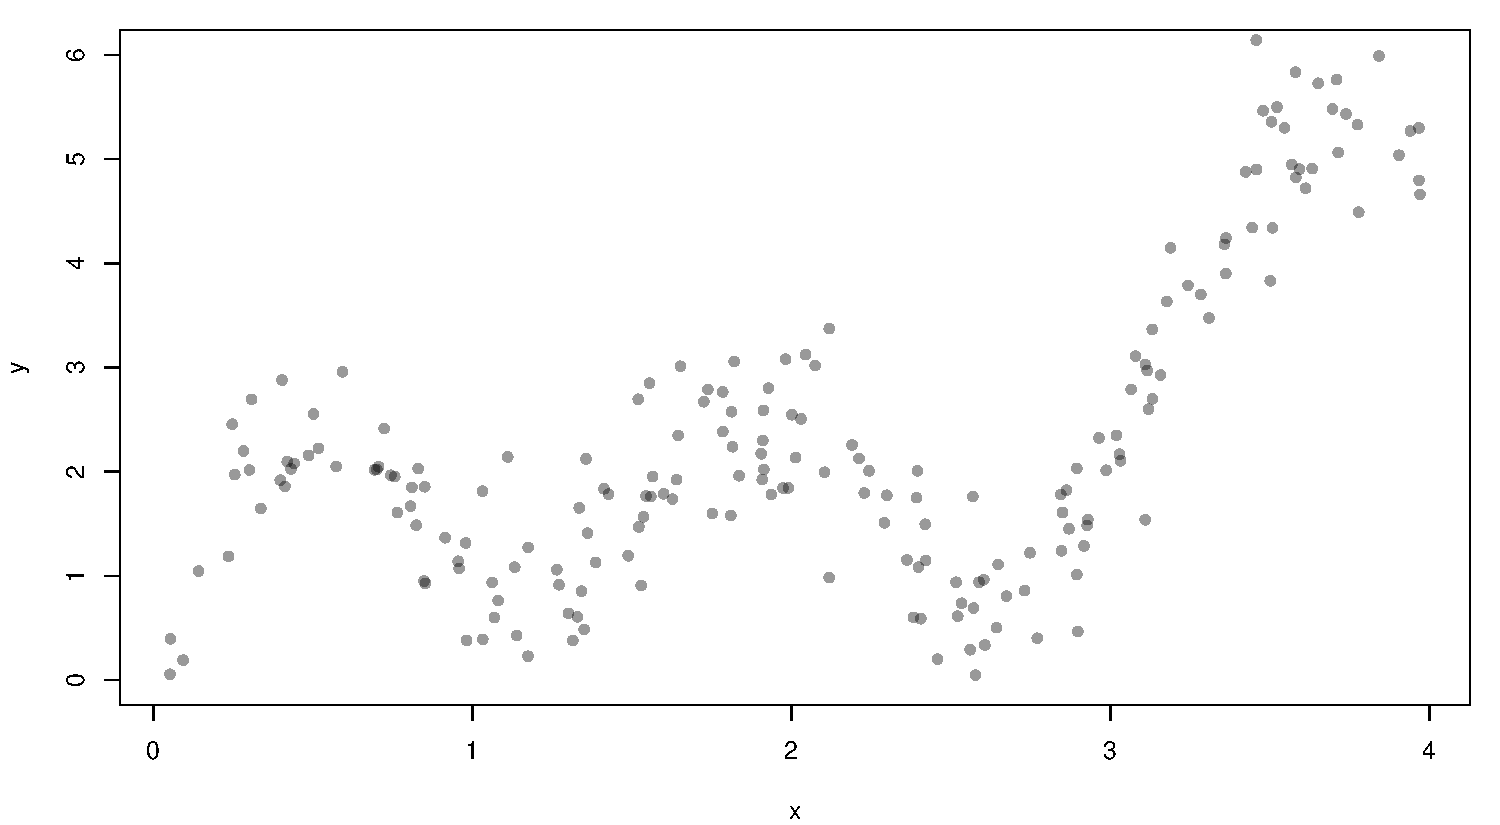
\includegraphics[width=\linewidth]{valid1.pdf}
%\end{center}
%
%\end{frame}
%
%%%%%%%%%%%%%%%%%%%%%%%%%%%%%%%%%%%%%%%%%%%%%%%%%%%%
%\begin{frame}[fragile] \frametitle{}
%
%\begin{center}
%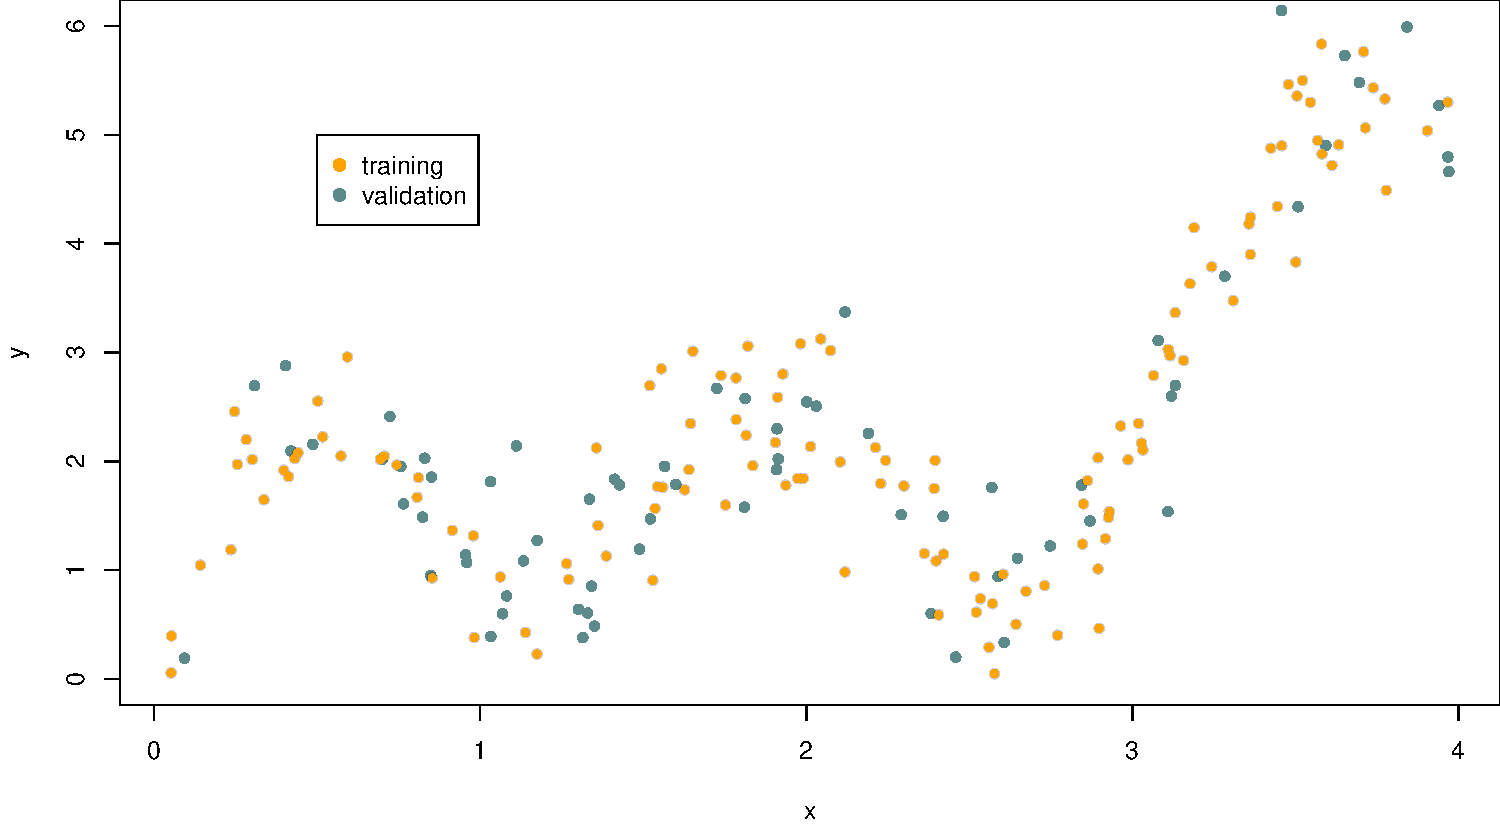
\includegraphics[width=\linewidth]{valid2.pdf}
%\end{center}
%
%\end{frame}
%
%%%%%%%%%%%%%%%%%%%%%%%%%%%%%%%%%%%%%%%%%%%%%%%%%%%%
%\begin{frame}[fragile] \frametitle{}
%
%\begin{center}
%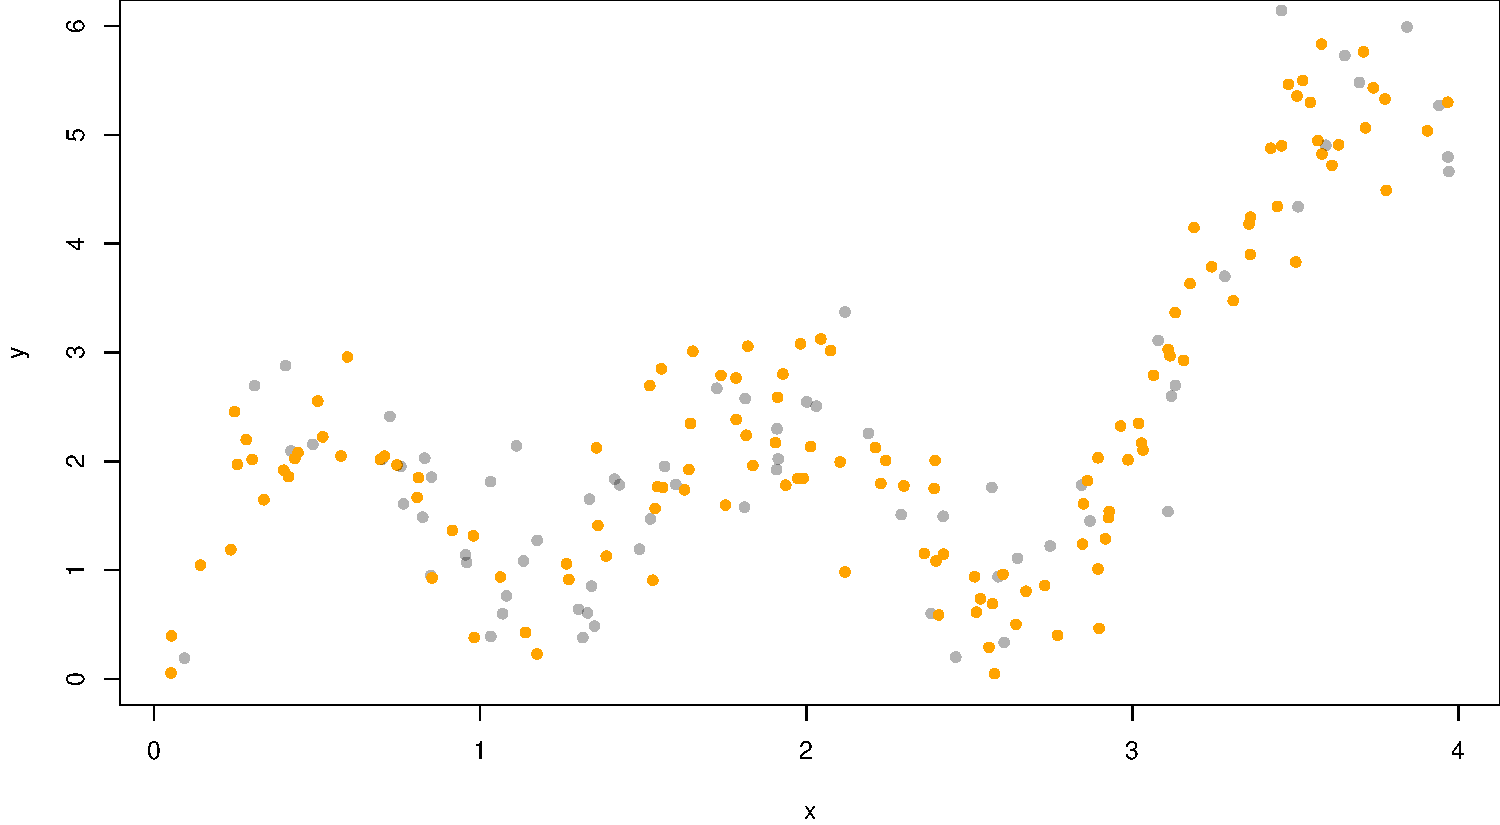
\includegraphics[width=\linewidth]{valid3.pdf}
%\end{center}
%
%\end{frame}
%
%%%%%%%%%%%%%%%%%%%%%%%%%%%%%%%%%%%%%%%%%%%%%%%%%%%%
%\begin{frame}[fragile] \frametitle{}
%
%\begin{center}
%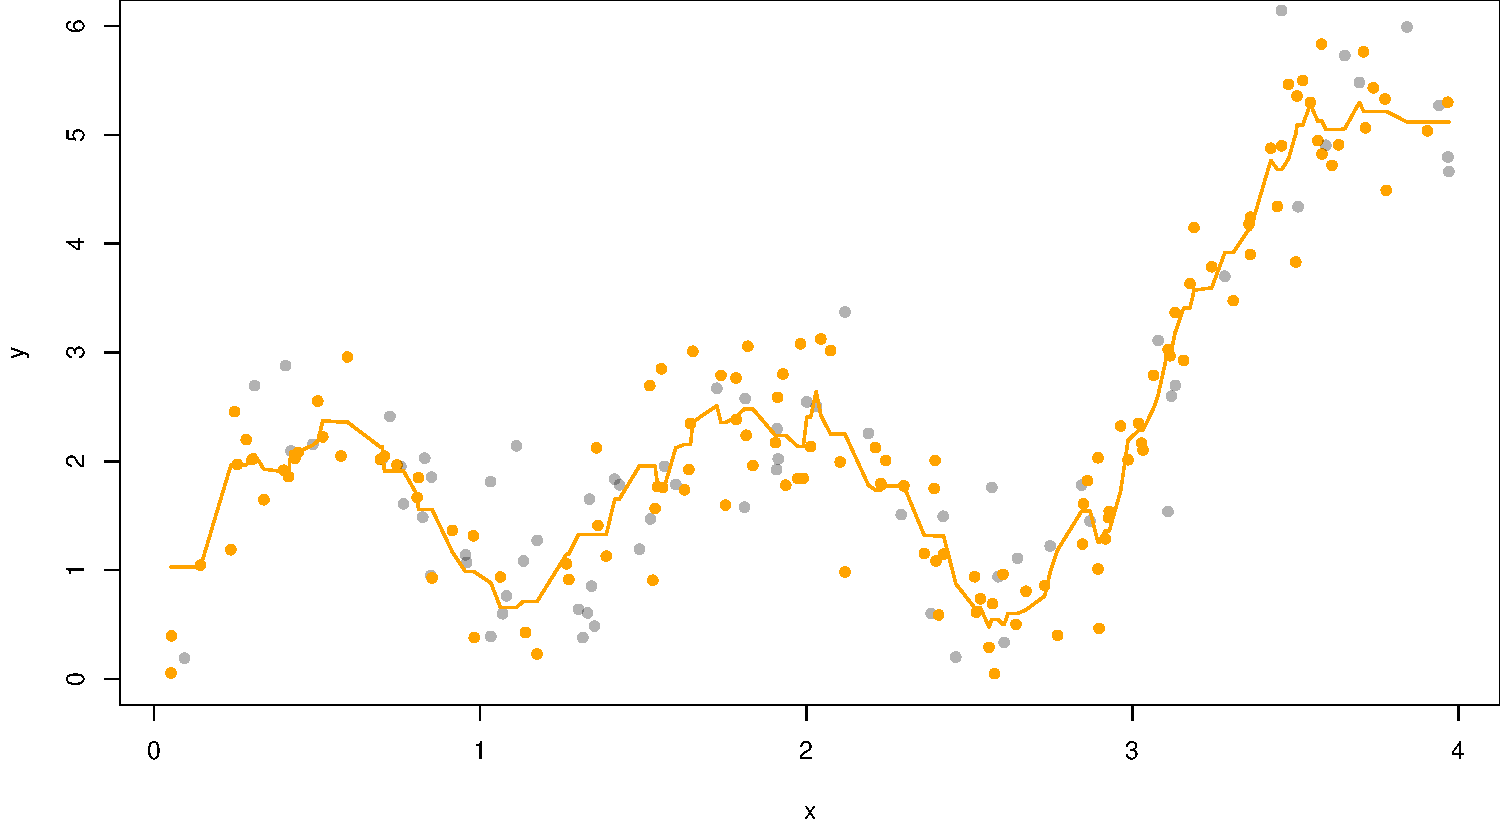
\includegraphics[width=\linewidth]{valid4.pdf}
%\end{center}
%
%\end{frame}
%
%%%%%%%%%%%%%%%%%%%%%%%%%%%%%%%%%%%%%%%%%%%%%%%%%%%%
%\begin{frame}[fragile] \frametitle{}
%
%\begin{center}
%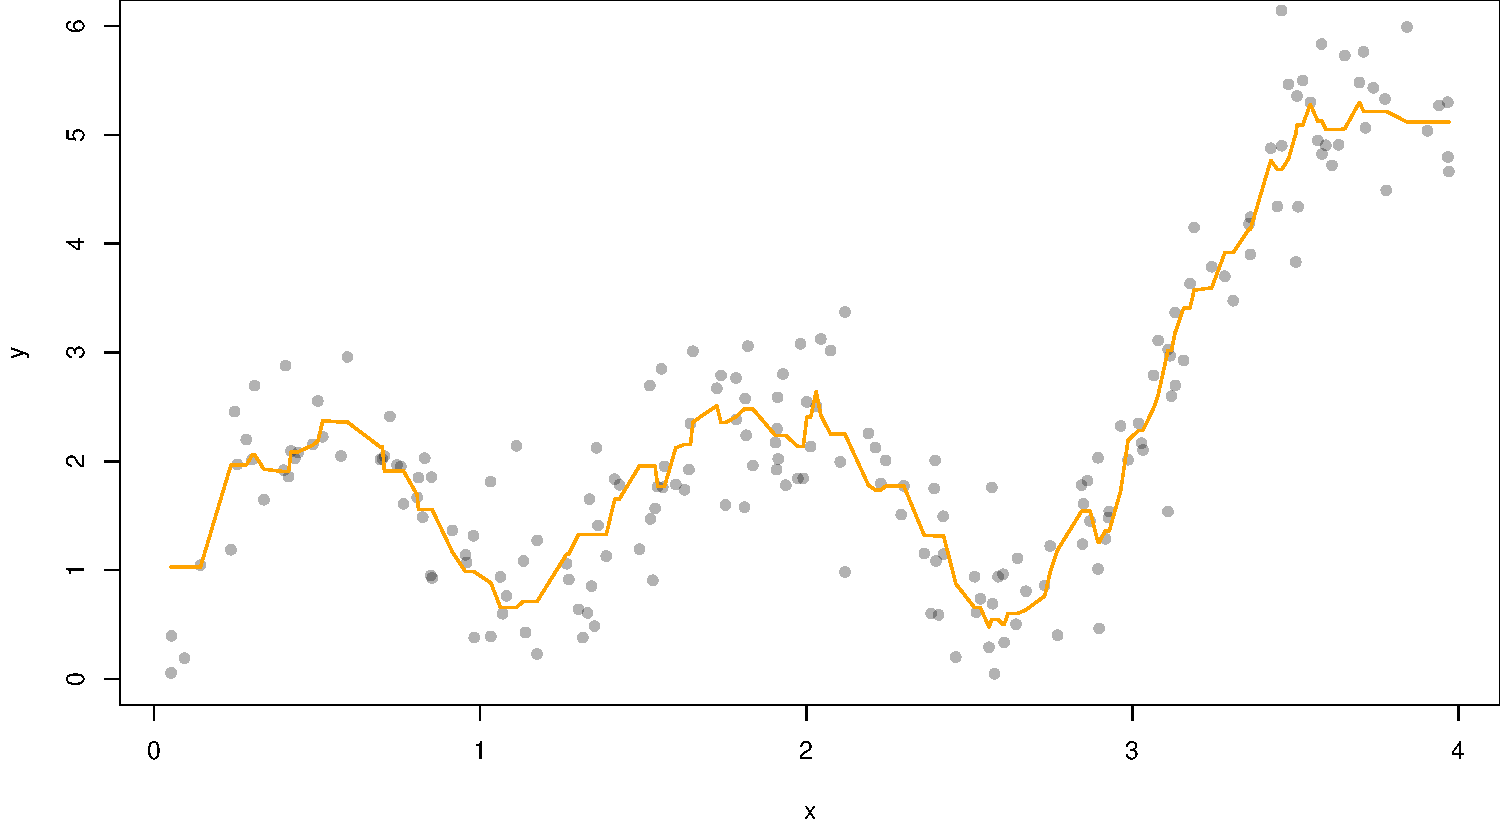
\includegraphics[width=\linewidth]{valid5.pdf}
%\end{center}
%
%\end{frame}
%
%%%%%%%%%%%%%%%%%%%%%%%%%%%%%%%%%%%%%%%%%%%%%%%%%%%%
%\begin{frame}[fragile] \frametitle{}
%
%\begin{center}
%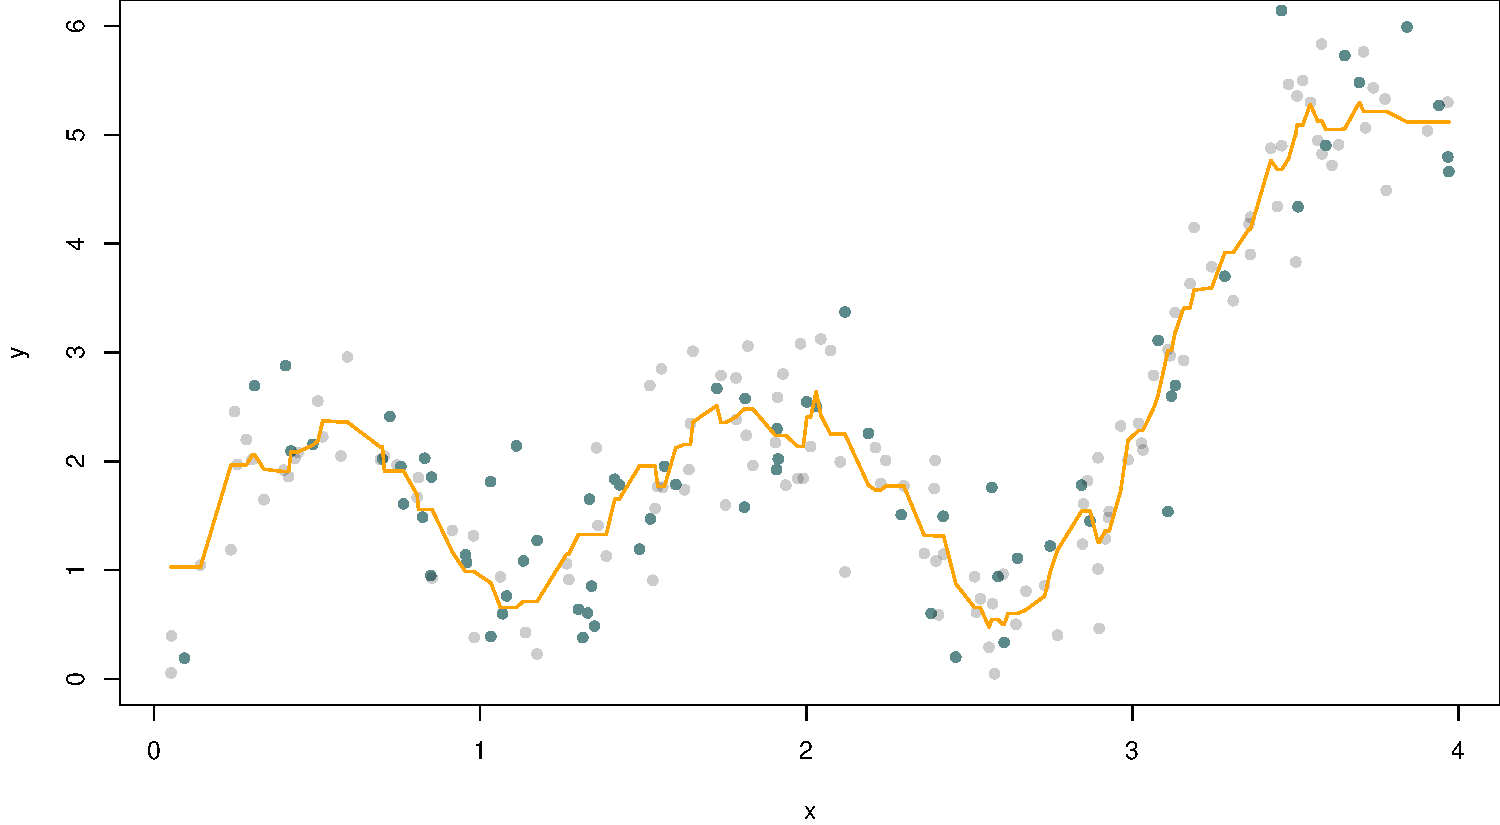
\includegraphics[width=\linewidth]{valid6.pdf}
%\end{center}
%
%\end{frame}
%
%%%%%%%%%%%%%%%%%%%%%%%%%%%%%%%%%%%%%%%%%%%%%%%%%%%%
%\begin{frame}[fragile] \frametitle{}
%
%\begin{center}
%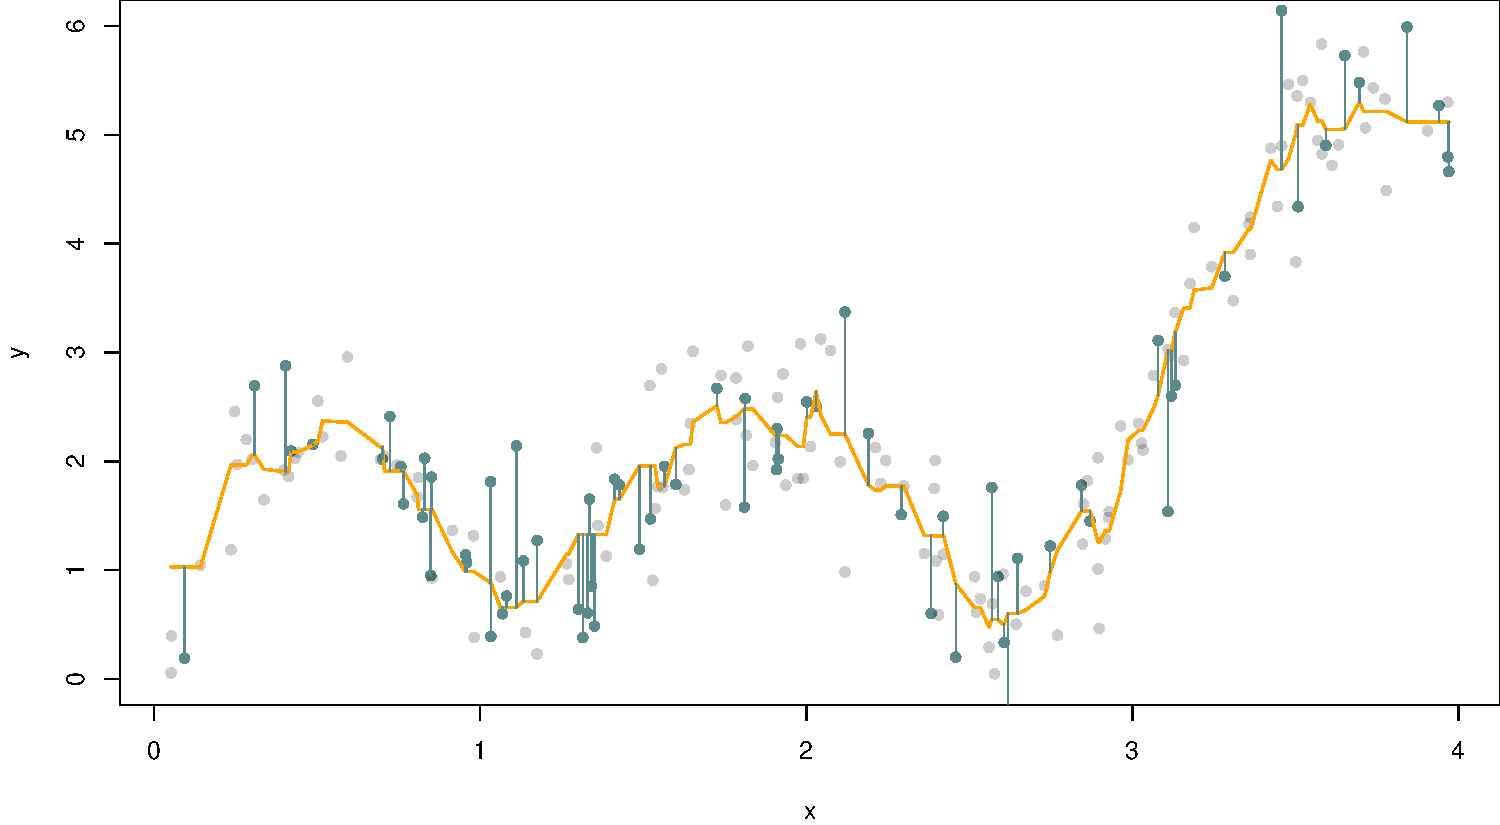
\includegraphics[width=\linewidth]{valid7.pdf}
%\end{center}
%
%\end{frame}
%
%%%%%%%%%%%%%%%%%%%%%%%%%%%%%%%%%%%%%%%%%%%%%%%%%%%%
%\begin{frame}[fragile] \frametitle{}
%
%\begin{flushright}
%{Depth}
%\end{flushright}
%
%\end{frame}
%
%%%%%%%%%%%%%%%%%%%%%%%%%%%%%%%%%%%%%%%%%%%%%%%%%%%%
%\begin{frame}[fragile] \frametitle{}
%
%So if shallow neural networks can represent arbitrary
%functions, why have we been creating deeper and deeper
%networks? A recent theoretical paper tries to explain
%why deeper networks perform significantly better:
%\begin{quote}
%Montufar, Guido F., et al. ``On the number of linear regions of deep neural networks." Advances in neural information processing systems. 2014.
%\end{quote}
%
%\end{frame}
%
%%%%%%%%%%%%%%%%%%%%%%%%%%%%%%%%%%%%%%%%%%%%%%%%%%%%
%\begin{frame}[fragile] \frametitle{}
%
%\begin{center}
%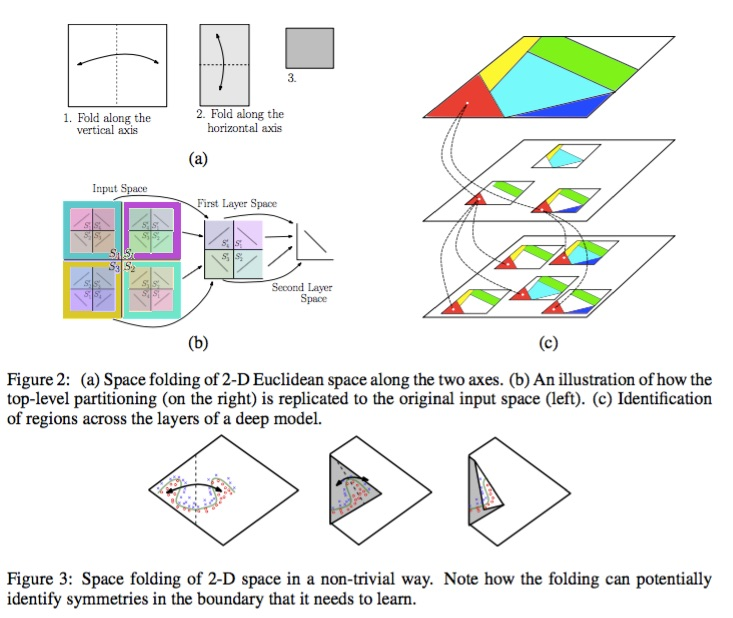
\includegraphics[height=8cm]{linearUnits.jpg}
%\end{center}
%
%\end{frame}
%
%%%%%%%%%%%%%%%%%%%%%%%%%%%%%%%%%%%%%%%%%%%%%%%%%%%%
%\begin{frame}[fragile] \frametitle{}
%
%A summary of one result from the paper: A dense
%neural network with rectified linear activations having
%$n_0$ input units and $L$ hidden layers of width $n \geq n_0$
%can compute function that have:
%\begin{align*}
%\Omega \left( \left(\frac{n}{n_0} \right)^{(L-1) \cdot n_0} n^{n_0} \right)
%\end{align*}
%Number of linear regions. This shows that the expressibility
%of the network grows exponentially with $L$ but only polynomially
%with $n$.
%
%So, deeper models approximate a larger class of functions with
%fewer parameters.
%
%\end{frame}
%
%%%%%%%%%%%%%%%%%%%%%%%%%%%%%%%%%%%%%%%%%%%%%%%%%%%%
%\begin{frame}[fragile] \frametitle{}
%
%\begin{center}
%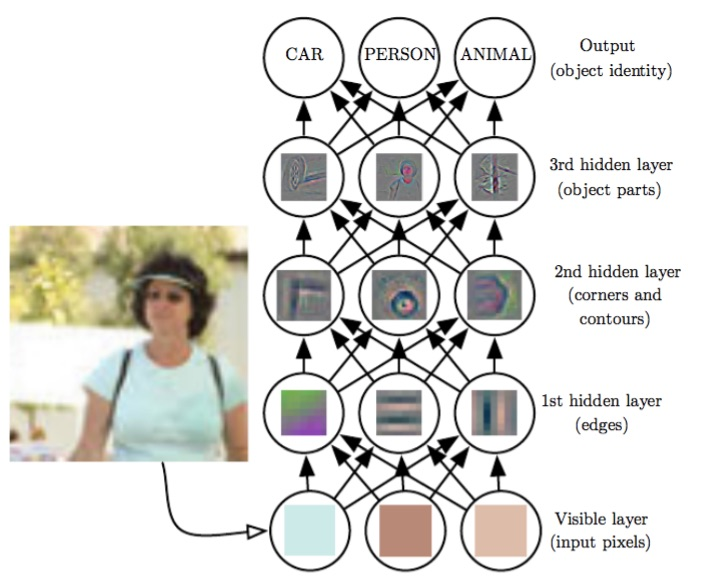
\includegraphics[height=8cm]{representation.jpg}
%\end{center}
%
%\end{frame}
%
%%%%%%%%%%%%%%%%%%%%%%%%%%%%%%%%%%%%%%%%%%%%%%%%%%%%
%\begin{frame}[fragile] \frametitle{}
%
%\begin{center}
%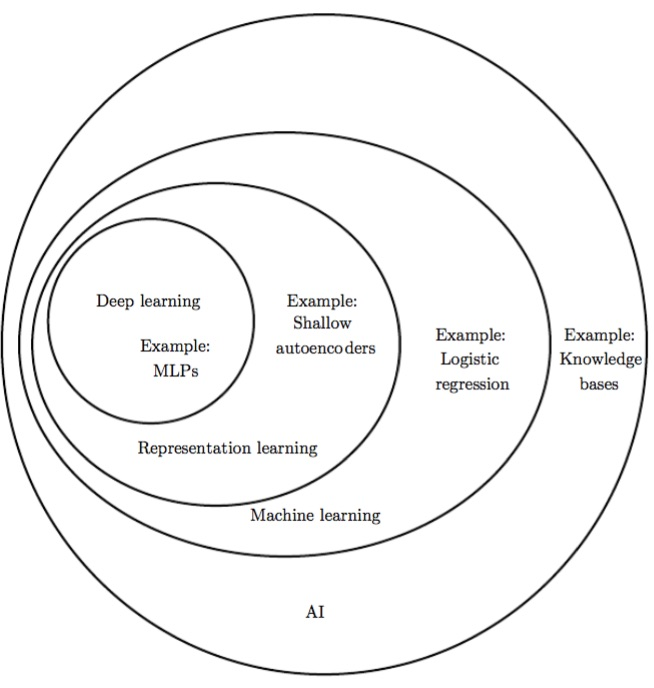
\includegraphics[height=8cm]{vennDiagram.jpg}
%\end{center}
%
%\end{frame}
%
%%%%%%%%%%%%%%%%%%%%%%%%%%%%%%%%%%%%%%%%%%%%%%%%%%%%
%\begin{frame}[fragile] \frametitle{}
%
%\begin{flushright}
%{Representation}
%\end{flushright}
%
%\end{frame}
%
%%%%%%%%%%%%%%%%%%%%%%%%%%%%%%%%%%%%%%%%%%%%%%%%%%%%
%\begin{frame}[fragile] \frametitle{}
%
%\begin{center}
%{I. Problem Set 8 part 1} \\
%{II. Problem Set 8, Part 2} \\
%{III. Transfer Learning: IMDB Sentiment analysis}
%\end{center}
%
%\end{frame}
%
%%%%%%%%%%%%%%%%%%%%%%%%%%%%%%%%%%%%%%%%%%%%%%%%%%%%
%\begin{frame}[fragile] \frametitle{}
%
%Neural networks have had amazingly successful results
%learning things such as basic mathematical operations:
%\begin{quote}
%Franco, Leonardo, and Sergio A. Cannas. "Solving arithmetic problems using feed-forward neural networks." Neurocomputing 18.1 (1998): 61-79.
%\end{quote}
%
%\end{frame}
%
%%%%%%%%%%%%%%%%%%%%%%%%%%%%%%%%%%%%%%%%%%%%%%%%%%%%
%\begin{frame}[fragile] \frametitle{}
%
%\begin{center}
%{IV. Learning addition}
%\end{center}
%
%\end{frame}
%
%%%%%%%%%%%%%%%%%%%%%%%%%%%%%%%%%%%%%%%%%%%%%%%%%%%%
%\begin{frame}[fragile] \frametitle{}
%
%There as also been work on using neural networks to
%capture subjective features such as painting style:
%\begin{quote}
%Gatys, Leon A., Alexander S. Ecker, and Matthias Bethge.
%"A neural algorithm of artistic style." arXiv preprint
%arXiv:1508.06576 (2015).
%\end{quote}
%
%\end{frame}
%
%%%%%%%%%%%%%%%%%%%%%%%%%%%%%%%%%%%%%%%%%%%%%%%%%%%%
%\begin{frame}[fragile] \frametitle{}
%
%\begin{center}
%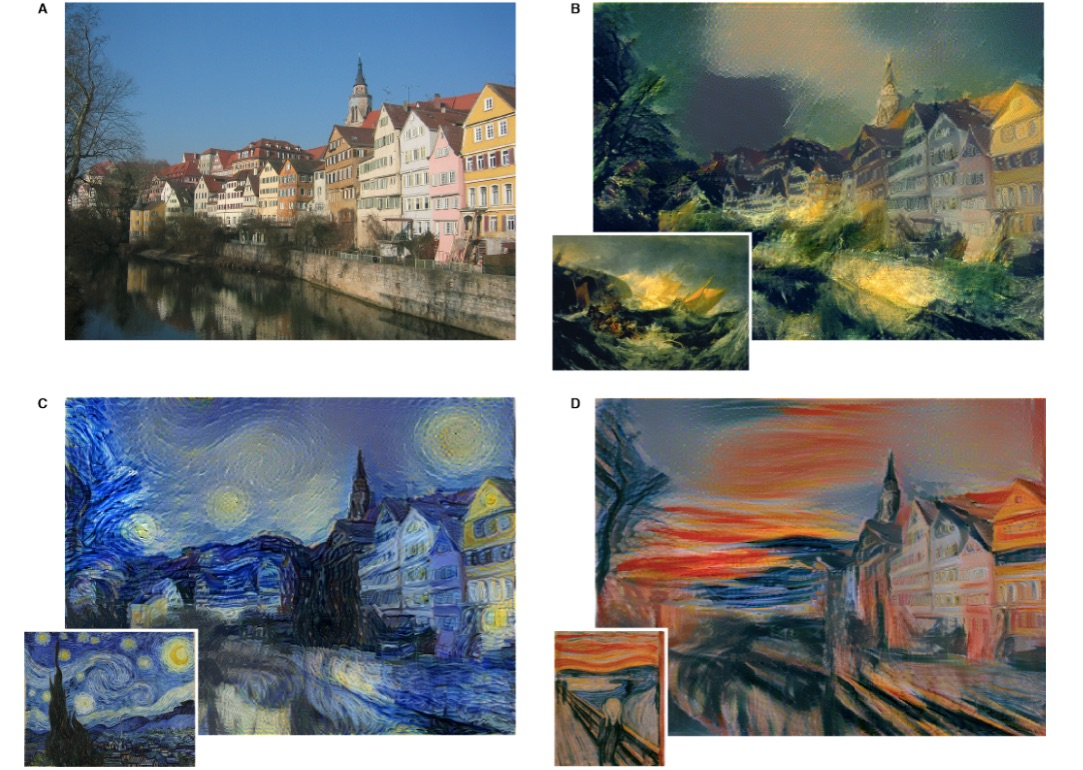
\includegraphics[height=8cm]{styleTransfer.jpg}
%\end{center}
%
%\end{frame}
%
%%%%%%%%%%%%%%%%%%%%%%%%%%%%%%%%%%%%%%%%%%%%%%%%%%%%
%\begin{frame}[fragile] \frametitle{}
%
%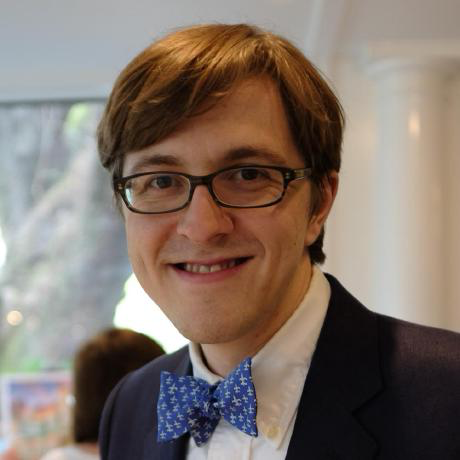
\includegraphics[width=0.4\linewidth]{me.png}
%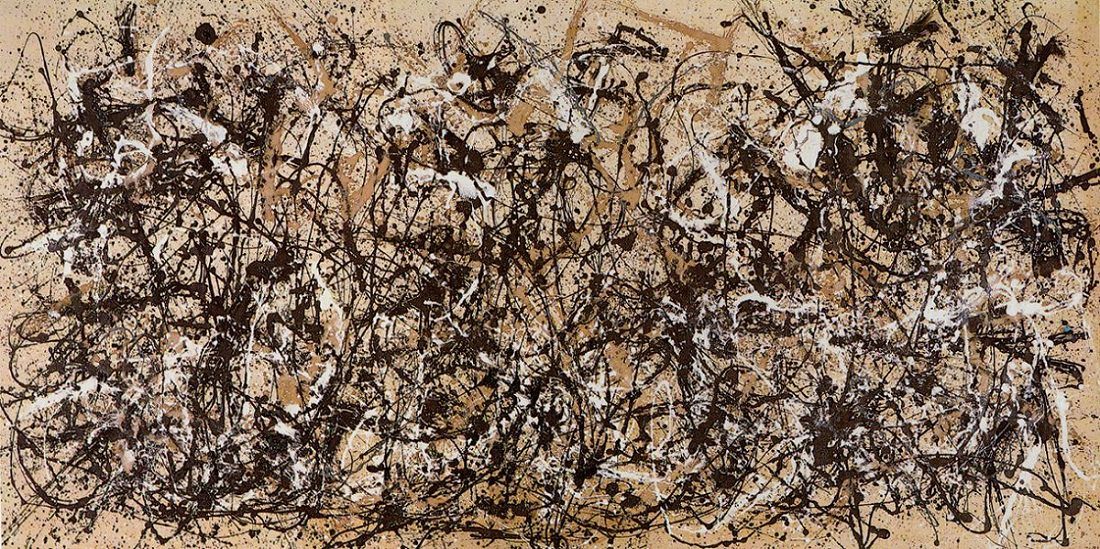
\includegraphics[width=0.5\linewidth]{pollock.jpg}
%
%\end{frame}
%
%
%%%%%%%%%%%%%%%%%%%%%%%%%%%%%%%%%%%%%%%%%%%%%%%%%%%%
%\begin{frame}[fragile] \frametitle{}
%
%\begin{center}
%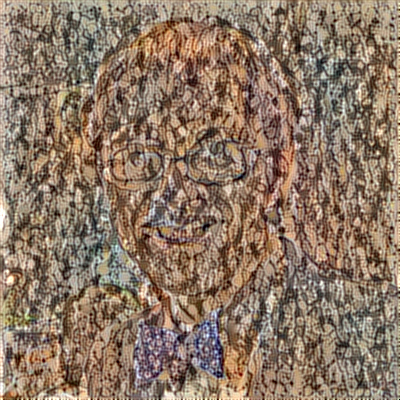
\includegraphics[width=0.6\linewidth]{me_pollock.png}
%\end{center}
%
%\end{frame}
%
%%%%%%%%%%%%%%%%%%%%%%%%%%%%%%%%%%%%%%%%%%%%%%%%%%%%
%\begin{frame}[fragile] \frametitle{}
%
%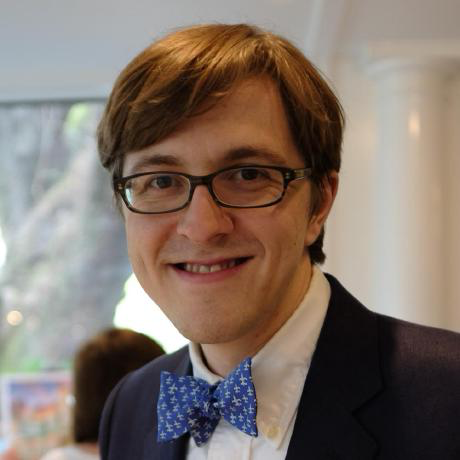
\includegraphics[width=0.4\linewidth]{me.png}
%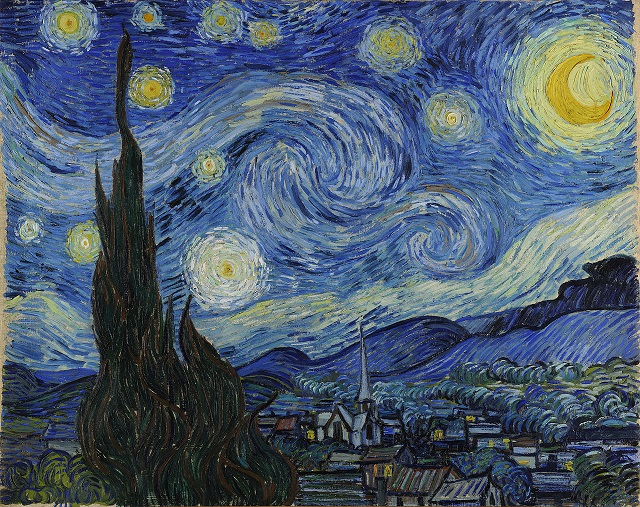
\includegraphics[width=0.5\linewidth]{stary.jpg}
%
%\end{frame}
%
%
%%%%%%%%%%%%%%%%%%%%%%%%%%%%%%%%%%%%%%%%%%%%%%%%%%%%
%\begin{frame}[fragile] \frametitle{}
%
%\begin{center}
%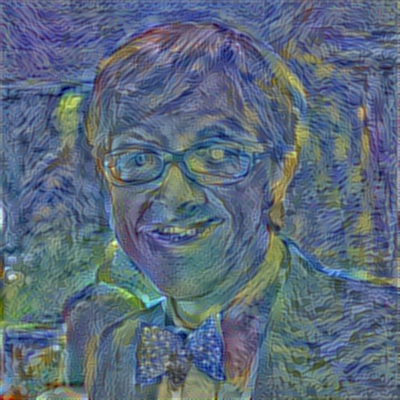
\includegraphics[width=0.6\linewidth]{me_stary.png}
%\end{center}
%
%\end{frame}
%
%%%%%%%%%%%%%%%%%%%%%%%%%%%%%%%%%%%%%%%%%%%%%%%%%%%%
%\begin{frame}[fragile] \frametitle{}
%
%\begin{flushright}
%{Future}
%\end{flushright}
%
%\end{frame}
%
%%%%%%%%%%%%%%%%%%%%%%%%%%%%%%%%%%%%%%%%%%%%%%%%%%%%
%\begin{frame}[fragile] \frametitle{}
%
%Near-term popular areas of study in deep learning:
%\begin{itemize}
%\item compression of neural networks
%\item consolidating the CNN tricks and tips; when will this
%ever slow down or end?
%\item deep residual neural networks
%\end{itemize}
%
%\end{frame}
%
%%%%%%%%%%%%%%%%%%%%%%%%%%%%%%%%%%%%%%%%%%%%%%%%%%%%
%\begin{frame}[fragile] \frametitle{}
%
%A robot at work:
%\begin{center}
%{\url{http://www.youtube.com/watch?v=2yRRNGr_4yY&t=1m0s}}
%\end{center}
%
%\end{frame}
%
%%%%%%%%%%%%%%%%%%%%%%%%%%%%%%%%%%%%%%%%%%%%%%%%%%%%
%{
%\setbeamertemplate{background}{\parbox[c][\paperheight][c]{\paperwidth}{\centering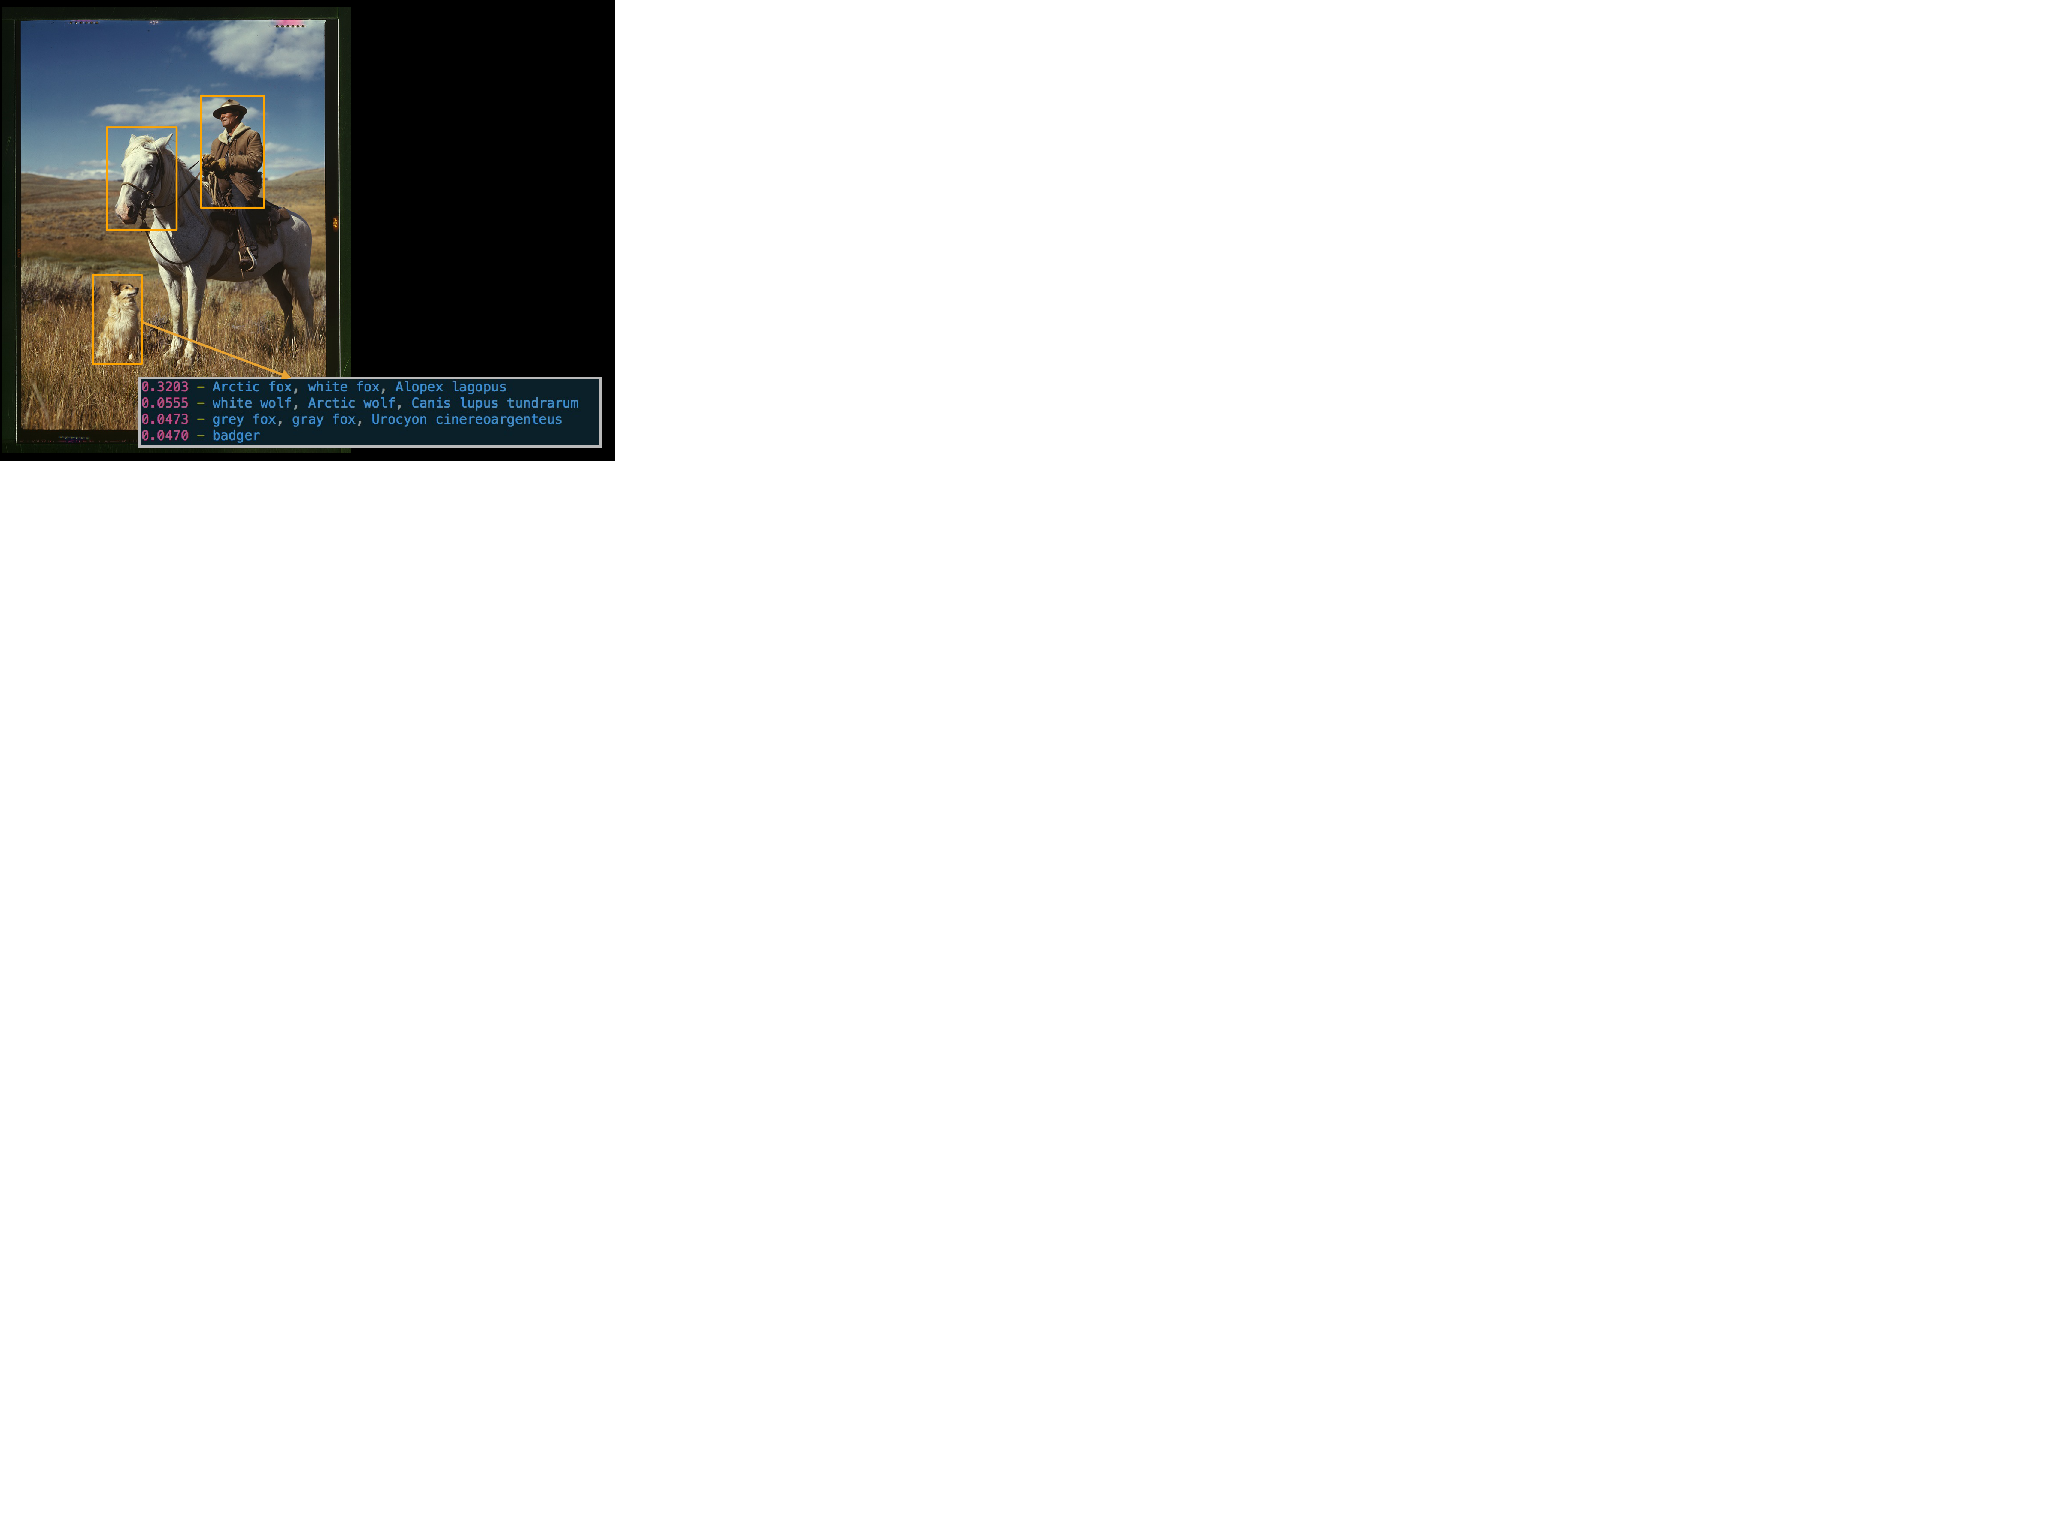
\includegraphics[width=0.7\paperwidth]{imageAnalysis1}}}
%\begin{frame}[plain]
%\end{frame}
%}
%
%%%%%%%%%%%%%%%%%%%%%%%%%%%%%%%%%%%%%%%%%%%%%%%%%%%%
%{
%\setbeamertemplate{background}{\parbox[c][\paperheight][c]{\paperwidth}{\centering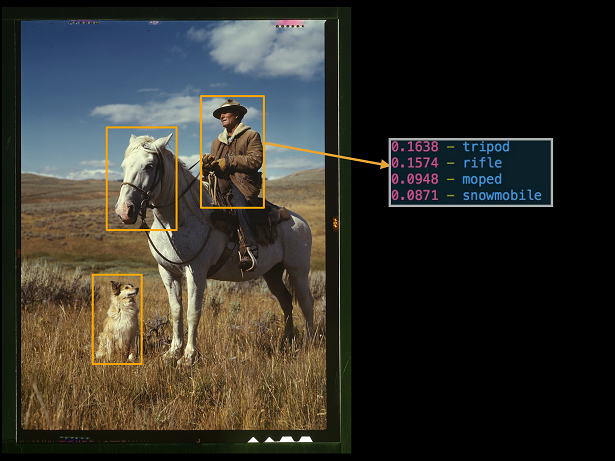
\includegraphics[width=0.7\paperwidth]{imageAnalysis2}}}
%\begin{frame}[plain]
%\end{frame}
%}
%
%%%%%%%%%%%%%%%%%%%%%%%%%%%%%%%%%%%%%%%%%%%%%%%%%%%%
%\begin{frame}[fragile] \frametitle{}
%
%To me, one of the more exciting papers on deep learning
%produced in the past year:
%\begin{quote}
%Gregor, K., Danihelka, I., Graves, A., \& Wierstra, D. (2015). DRAW: A recurrent neural network for image generation. arXiv preprint arXiv:1502.04623.
%\end{quote}
%It makes meaningful departures from prior methods and gets
%more directly at the generative model. It is also closer to
%our understanding of how visual processing happens in the
%brain.
%
%\end{frame}
%
%%%%%%%%%%%%%%%%%%%%%%%%%%%%%%%%%%%%%%%%%%%%%%%%%%%%
%\begin{frame}[fragile] \frametitle{}
%
%\begin{center}
%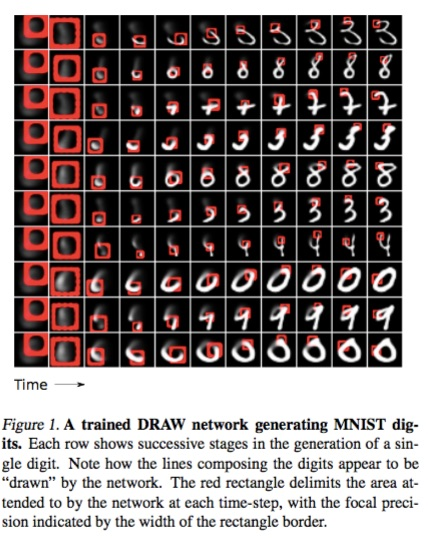
\includegraphics[width=0.5\linewidth]{draw.jpg}
%\end{center}
%
%\end{frame}

%%%%%%%%%%%%%%%%%%%%%%%%%%%%%%%%%%%%%%%%%%%%%%%%%%%
\begin{frame}[fragile] \frametitle{}

Longer-term areas in deep learning:
\begin{itemize}
\item deep reinforcement learning
\item better architectures or training algorithms
\item (real) unsupervised learning
\end{itemize}

\end{frame}

%%%%%%%%%%%%%%%%%%%%%%%%%%%%%%%%%%%%%%%%%%%%%%%%%%%%
%\begin{frame}[fragile] \frametitle{}
%
%\begin{center}
%{\color{yaleblue}\sc\fontsize{2cm}{0cm}\selectfont Thanks!}
%\end{center}
%
%\end{frame}


%
%
%\end{document}
%
%%%% Local Variables:
%%%% mode: latex
%%%% TeX-master: t
%%%% End:
